
% ===========================================================================
% Title:
% ---------------------------------------------------------------------------
% to create Type I fonts type "dvips -P cmz -t letter <filename>"
% ===========================================================================
\documentclass[11pt]{article}       %--- LATEX 2e base
\usepackage{latexsym}               %--- LATEX 2e base
%---------------- Wide format -----------------------------------------------
\textwidth=6in \textheight=9in \oddsidemargin=0.25in
\evensidemargin=0.25in \topmargin=-0.5in
\linespread{2}
%--------------- Algorithm --------------------------------------------------
\newtheorem{algX}{Algorithm}
\newenvironment{algorithm}       {\begin{algX}\begin{em}}%
                                 {\par\noindent --- End of Algorithm ---
                                 \end{em}\end{algX}}
\newcommand{\step}[2]            {\begin{list}{}
                                  {  \setlength{\topsep}{0cm}
                                     \setlength{\partopsep}{0cm}
                                     \setlength{\leftmargin}{0.8cm}
                                     \setlength{\labelwidth}{0.7cm}
                                     \setlength{\labelsep}{0.1cm}    }
                                  \item[#1]#2    \end{list}}
                                 % usage: \begin{algorithm} \label{xyz}
                                 %        ... \step{(1)}{...} ...
                                 %        \end{algorithm}
%--------------- Figures ----------------------------------------------------
\usepackage{graphicx}

\newcommand{\includeFig}[3]      {\begin{figure}[htb] \begin{center}
                                 \includegraphics
                                 [width=4in,keepaspectratio]
                                 {#2}\caption{\label{#1}#3} \end{center} \end{figure}}
                                 % usage: \includeFig{label}{file}{caption}


% ===========================================================================
\begin{document}
% ===========================================================================

% ############################################################################
% Title
% ############################################################################

\title{CUDA-accelerated Genetic Feedforward-ANN Training for Data Mining}


% ############################################################################
% Author(s) (no blank lines !)
\author{
% ############################################################################
Catalin Patulea, Robert Peace, and James Green\\
School of Systems and Computer Engineering\\
Carleton University\\
Ottawa, Canada K1S 5B6\\
{\em cat@vv.carleton.ca}, {\em rpeace@sce.carleton.ca}, {\em jrgreen@sce.carleton.ca}
% ############################################################################
} % end-authors
% ############################################################################

\maketitle

% ############################################################################
% Abstract
% ############################################################################
\begin{abstract}
We present an implementation of genetic algorithm (GA) training of feedforward artificial neural networks (ANNs) targeting commodity graphics cards (GPUs). By carefully mapping the problem onto the unique GPU architecture, we achieve order-of-magnitude speedup over a conventional CPU implementation. Furthermore, we show that the speedup is consistent across a wide range of data set sizes, making this implementation ideal for large data sets. This performance boost enables the genetic algorithm to search a larger subset of the solution space, which results in more accurate pattern classification. Finally, we demonstrate this method in the context of the 2009 UC San Diego Data Mining Contest, achieving a world-class lift on a data set of 94682 e-commerce transactions.
\end{abstract}

% ############################################################################
\section{Introduction} \label{intro}
% ############################################################################
Genetic algorithms (GAs) are a stochastic, evolutionary approach to machine learning for pattern classification. While greedy methods will get stuck at local extrema, GAs  are theoretically capable of asymptotically reaching the global optimum \cite{GA-ANN}. However, because they require the evaluation of approximately 50 to 100 classifiers at each iteration, and the algorithm is repeated for several thousand iterations, they are extremely compute-intensive. This is exacerbated by the use of artificial neural networks (ANNs) as the classifier because ANNs themselves are very compute-intensive.

Compared to a traditional sequential implementation of GA training of ANNs, the use of graphical processing units (GPUs) as parallel processors provides significant performance improvements at a fraction of the price of alternatives such as cluster computing. GPUs, however, use a specialized programming paradigm which must be taken into account to leverage their full processing power. In this report, we show an implementation of GA training of ANNs which achieves an order-of-magnitude speedup over a sequential algorithm.

% ############################################################################
\section{Background} \label{background}
% ############################################################################

% ----------------------------------------------------------------------------
\subsection{Artificial Neural Networks} \label{ann}
% ----------------------------------------------------------------------------
ANNs are composed of nodes connected by weighted directed edges. In a feed-forward network architecture, nodes are organized into an input layer, one or more hidden layers, and an output layer. Each layer is fully connected to the next. Figure~\ref{fig:ann-chromosome} demonstrates the feedfoward ANN structure. Each of the hidden nodes at hidden layer $n$ perform a transcendental function with inputs equal to the outputs of layer $n-1$ each multiplied by the weight associated with the edge through which they are fed from layer $n-1$ to layer $n$. In a radial basis function (RBF) network, the nodes in each hidden layer calculate the distance between their inputs and a centre vector, and pass a weighted distance to a RBF. Nodes in a sigmoid function network perform a similar operation with a sigmoid function in place of the RBF. The output node is typically linear, computing a weighted sum of its inputs. The output of the ANN is a single real value which is interpreted as a classification confidence. ANN computation is dominated by the number of multiplications at the directed edges, proportional to the number of features in the data set and the number of hidden nodes, and by the transcendental functions at the hidden nodes, which are typically exponentiations.  ANN training has been implemented previously on GPU hardware, however these efforts have focused on training through backpropagation \cite{backprop} as opposed to genetic algorithms.

% ----------------------------------------------------------------------------
\subsection{Genetic Algorithms as ANN Training Agents} \label{ga}
% ----------------------------------------------------------------------------
Genetic algorithms (GAs) use populations of candidate solutions to simultaneously explore the search space of ANN parameters \cite{GA-ANN}. The candidate ANNs are randomly mutated, mated and selected during each of several generations. Mutation and mating is done using a problem-specific representation of candidate solutions and "genetic operators." Selection requires calculating the fitness of each candidate ANN  then preferentially selecting candidate ANNs based on fitness. The fitness of a classifier is a classifier accuracy metric such as sensitivity.  The competitive bias imposed by selection attempts to mimic the "survival of the fittest" principle often seen in nature.  Because GAs perform an unbiased search of a solution space and ANNs can be of arbitrary complexity, this technique is suitable for data mining applications using large or complex data sets.

The computation required for GA training of ANNs is proportional to the number of generations ($10^1$-$10^4$), to the size of each generation ($10^1$-$10^2$ candidates) and to the size of the data set ($10^2$-$10^6$ instances).

% ----------------------------------------------------------------------------
\subsection{The CUDA Platform} \label{cuda}
% ----------------------------------------------------------------------------
NVidia's Compute Unified Device Architecture (CUDA) is a programming platform for massively parallel GPUs found in off-the-shelf graphics cards. GPUs consist of several dozen independent floating-point units, providing significant speedup to data-parallel compute-intensive applications \cite{cuda}. Each unit is connected to on-board memory using a very wide bus, enabling high memory bandwidth provided certain memory access rules are respected. These features make CUDA an ideal platform for GA-ANN training.

% ----------------------------------------------------------------------------
\subsection{Sample Application} \label{contest}
% ----------------------------------------------------------------------------
Our demonstration classifier is designed for the 2009 UC San Diego Data Mining Contest "E-commerce Transaction Anomaly Classification" \cite{UCSG-Contest} and with training data thereof. The training data consist of 94682 instances with 19 features of mixed types and a 1:50 binary class imbalance. The evaluation metric is "lift at 20\%", which can be understood as the ratio of the true positive rate in the top 20\% ranked instances to the overall positive rate of the data set.  Lift at 20\% is commonly used in marketing research in order to select the subset of a population which is most likely to respond to solicitation.

% ############################################################################
\section{Classifier Design} \label{design}
% ############################################################################

% ----------------------------------------------------------------------------
\subsection{ANN Structure Design} \label{ann}
% ----------------------------------------------------------------------------

While our GA-ANN classifier was designed for the 2009 UC San Diego Data Mining Contest data set, it has been designed in order to be capable of adapting to a variety of data sets.  We have developed a flexible ANN topology, allowing for either one or two layers of hidden nodes and an arbitrary number of hidden nodes per layer (within the limits of GPU memory). In addition, each layer of the ANN is capable of performing RBF or sigmoid calculations.

The classifier receives as inputs real-valued features which are standardized prior to processing by the ANN.  The classifier outputs a single real value, in the range of 0 and 1, which represents the confidence with which the pattern is a member of the positive class.  These confidence values can be used for ranking during lift calculations, or for sensitivity or specificity measures with an arbitrary value chosen as a threshold for positive identification of a pattern.  Therefore, the fitness function is not limited to lift at 20\% as presented in this report.

% ----------------------------------------------------------------------------
\subsection{Genetic Algorithm Design} \label{ann}
% ----------------------------------------------------------------------------

For a single-layer ANN, as used in our final design, each candidate ANN is represented by a chromosome which consists of four arrays of real-valued numbers. Edge weights between input nodes and hidden layers, edge weights between hidden and output layers, width values for RBFs at hidden nodes and center values for RBFs at hidden nodes are all encoded, and can take on any real value. Figure~\ref{fig:ann-chromosome} demonstrates the chromosome structure and its relation to ANN structure.  This structure is simple yet powerful; individual edges are 'removed' by the genetic algorithm when their weight is set to zero and nodes are 'removed' by the genetic algorithm when their RBF width value is set to zero.  Thus, while the topology of the ANN is limited to those with $m$ layers and $n$ nodes per layer, the genetic algorithm searches all topologies with $m$ layers and between 0 and $n$ nodes per layer.

\begin{figure}[h]
	\centering
	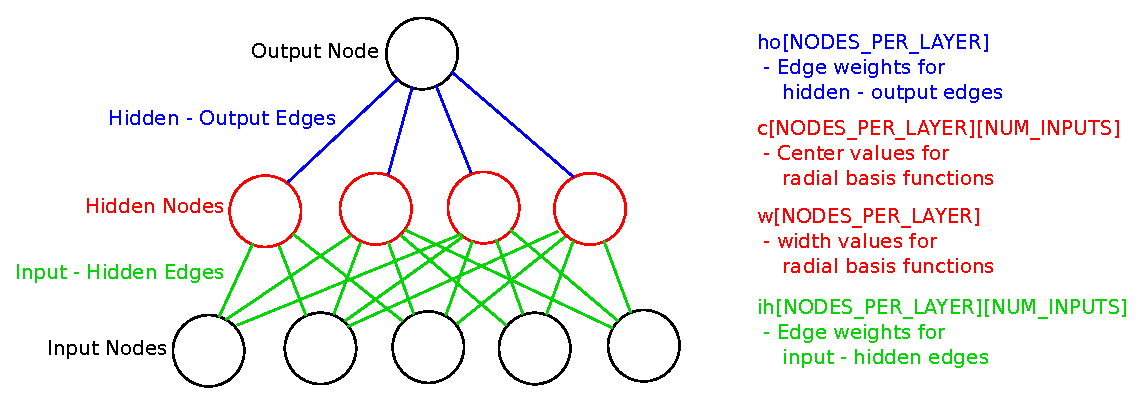
\includegraphics[width=\textwidth]{ann-chromosome}
	\caption{ANN structure and related chromosome design.  Each element in the chromosome is a real-valued number.}
	\label{fig:ann-chromosome}
\end{figure}

The genetic mutation and crossover operations which we have implemented are based on the methods defined by Montana and Lawrence \cite{GA-ANN}. Of the operations presented in this paper, the MUTATE NODES and CROSSOVER WEIGHTS operations were determined to provide an optimal balance between performance and classifier accuracy, and have been implemented in all of our experiments.

% ----------------------------------------------------------------------------
\subsection{Preliminary Data Analysis} \label{prelim}
% ----------------------------------------------------------------------------
To get a first idea of the separability of the data, we took an approach similar to Fisher's linear discriminant. This discriminant finds the 1D projection of the data which maximizes class separation, defined as the ratio of between-class variance and within-class variance. The problem of finding Fisher's linear discriminant can be seen as a generalized eigenvalue problem where the eigenvector with the large eigenvalue is the desired projection \cite[\S 3.8.2]{Duda}.
To gain more insight into the higher-dimensional properties of the data, and because 2D visualization is practical, we instead used the eigenvectors with the \emph{two} highest eigenvalues and formed a 2D projection of the data (Figure~\ref{fig:fishers-2d}). The resulting four approximately-Gaussian clusters guided our decision to use a radial basis function network with four Gaussian hidden nodes.

\begin{figure}[h]
	\centering
	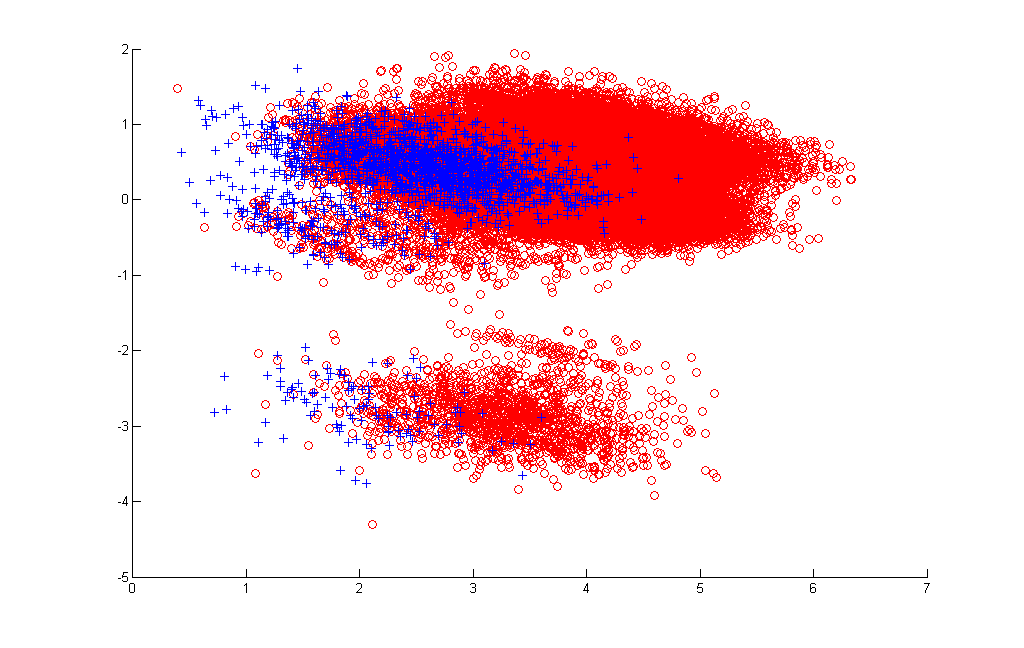
\includegraphics[width=\textwidth]{fishers_2d}
	\caption{Projection of original data set on hyperplane formed by the two eigenvectors with the largest eigenvalues.}
	\label{fig:fishers-2d}
\end{figure}

% ----------------------------------------------------------------------------
\subsection{Data Preprocessing Steps} \label{preprocessing}
% ----------------------------------------------------------------------------
In order to handle nominal feature values in data sets, we have implemented an algorithm which, given a tab seperated values file, converts nominal feature values in the data set into numeric values.  The algorithm replaces each nominal value in the data set with the logarithm of the probability ratio between the positive and negative classifications observed given the nominal value.  As a result, meaningful numeric values can be extracted from nominal values without domain knowledge relating to the values. This improves on the traditional orthogonal coding method \cite[slide 17]{MLP-NominalCoding} by avoiding allocation of a disproportionate number of input nodes to nominal features.  The logarithm of the ratio of all positive classifications to all negative classifications is attributed to nominal values which do not appear sufficiently in the data set and for values which appear only in blind test data sets; this prevents the classifier from attributing significant values to nominal values for which little or no inference can be done.

Due to the inherent limitations of floating-point (FP) representation of real values, the range of inputs to the ANN plays a crucial part in the numerical stability of the classifier during training and during classification. In particular, our use of exponential functions resulted in an ANN very sensitive to output saturation. In these cases, while the input to the \texttt{expf} function is well within the range of representible FP numbers (take for example feature 11 which has a maximum of 8193), the mathematical output of the exponentiation is too large to be represented in FP. This causes degenerate output values such as infinity or NaN (not a number). These special values propagate through the ANN edges to produce degenerate values at the output of the classifier.

To avoid this issue, we standardize the data before training and before classification. For each feature individually, we estimate the 10\textsuperscript{th} and 90\textsuperscript{th} percentiles of the feature values. Then we shift and scale the values such that 80\% of the resulting values are found between -1 and 1. This standardization method was chosen for its robustness against outliers. After standardization, the range of inputs to \texttt{expf} is narrow enough to always produce a valid FP value at the output. The standardization does not affect the classification itself because there are scaling and shifting parameters within the ANN (input to hidden edge weights and hidden center parameters, respectively) which are already part of the search space.

% ############################################################################
\section{Implementation of GA Training of ANNs} \label{algimp}
% ############################################################################

Our GA begins by generating an initial population of random candidate ANNs, each of which is a set of parameters describing one ANN. Feature values for all training instances are loaded into GPU global memory in preparation for ANN computations. Then, the following steps are executed in sequence for each generation of the GA:

\begin{enumerate}
	\item Compute the ANN output corresponding to each training instance, as calculated by each candidate ANN in the population.
	\item Find the threshold that defines the highest 20\% outputs for each candidate's set of output values.
	\item Compute the number of top 20\% instances which are truly positive, again for each candidate ANN. This allows us to calculate lift, which is used as the fitness value for each candidate ANN.
	\item Apply genetic operators: mating, mutation and selection. The selected candidate ANNs become the new population, to be used in the next generation.
\end{enumerate}

Items 1, 2 and 3 were all implemented on the CUDA platform and are described in detail below. Performance results are given as the combined time for one generation of these three items but exclude one-time initialization. Item 4 is not very computationally intensive and was not parallelized. 

% ----------------------------------------------------------------------------
\subsection{Computation of ANN Output Values} \label{ANNcomp}
% ----------------------------------------------------------------------------
ANN output values are computed by reading the training instances as real-valued feature vectors and applying the appropriate operations represented by the network topology and parameters. Feature data are organized to efficiently use memory bandwidth. ANN output calculation is particularly well-suited to the CUDA architecture because it has a very high ratio of mathematical operations to memory accesses (160 multiplications, 4 exponentiations and 80 bytes of memory accesses for our ANN topology). In addition, each output value depends only on the current ANN parameters and one training instance's feature values. Therefore, parallelization of this step scales particularly well with hardware capabilities.

% ----------------------------------------------------------------------------
\subsection{Calculation of Top 20\% Threshold} \label{top20}
% ----------------------------------------------------------------------------
Next, we must calculate the $k^{th}$ largest value in each candidate's list of output values, where $k = 0.20 * n$ and $n$ is the number of output values (number of training instances). We can accomplish this by iterating through all $n$ unsorted output values and inserting each into a binary minheap of fixed size $k$. The heap size is kept fixed by removing the root (smallest node) after each insertion. At the end of this process, the root of the heap is the $k^{th}$ largest output value. The insertion and removal can be combined into a single operation which costs $O(\log k)$ time. The heap occupies $4 * k$ bytes of device shared memory.

Because fast on-chip memory (16~KB) is not large enough for our value of $k$ ($4 * 18936 =$ 74~KB), we instead use $p$ passes of $\frac{k}{p}$-sized heaps. Each pass examines only values which are less than the threshold calculated by the preceeding pass. For example, the third pass examines only values below the 10\% threshold and finds the top 5\% threshold of this subset of values. This threshold therefore is the 15\% threshold of the full list. The threshold calculated by the last pass is the desired 20\% threshold.

The overall complexity of our algorithm is $O(np \log \frac{k}{p})$. Each top 20\% calculation is performed independently for each candidate ANN. Therefore, the parallel performance of this step scales with hardware capabilities when there are enough candidates to occupy the entire device.

% ----------------------------------------------------------------------------
\subsection{Computation of Number of Truly Positive Top 20\% Instances} \label{truepos}
% ----------------------------------------------------------------------------
To compute the number of truly positive instances in the top 20\% of scores, if training instances are unsorted, we must read from memory each instance's true class and corresponding ANN output value and compare the output value to the candidate's threshold. For $n$ training instances, this requires $2 * n$ memory accesses. However, by keeping the $n_p$ positive instances first in memory, we need only read the first $n_p$ ANN outputs, knowing that they correspond to the positive instances. This reduces the number of memory accesses to $n_p$, which is significant particularly for training data with low positive rate (in our case, $2 * n = 189364$ while $n_p = 2080$). Sorting the training instances by class is a cheap operation which is performed only once during initialization and can be done by the host CPU.

Counting of positive instances above the candidate's threshold is performed independently, in parallel, for each candidate. However, because there may not be enough candidates to fully occupy the GPU, we also split the counting process for each candidate into 256 independent sub-counts: the first sub-counter processes training instances 0, 256, 512, \ldots, the second sub-counter instances 1, 257, 513, \ldots, such that the sub-counts can be executed in parallel. The striped assignment of training instance indices to sub-counters is necessary to take advantage of the full memory bandwidth of the GPU. The host CPU then aggregates the sub-counts by summing, which is a very lightweight operation.

Finally, each count is divided by the number of positive instances to give a positive rate in the top 20\%. Then, the ratio of this positive rate to the overall positive rate is the lift of each candidate. These operations are also comparatively lightweight and executed on the host CPU.

% ############################################################################
\section{Results} \label{results}
% ############################################################################
We first present the computational performance of our algorithm for classifier training, followed by the estimated classification performance of the classifier designed for the UC San Diego data mining contest.

% ----------------------------------------------------------------------------
\subsection{Experimental Setup} \label{experiment}
% ----------------------------------------------------------------------------
To evaluate the performance of our system, we compared execution time of equivalent algorithms running on commodity desktop CPUs and GPUs. Each series represents one type of experimental hardware (Table~\ref{tab:experimental-hardware}). Each data point is an average over 10 runs of the algorithm with the same parameters.

\begin{table}[h]
	\centering
	\begin{tabular}{lllll}
	\textbf{Legend Label} & \textbf{Hardware} & \textbf{Clock} & \textbf{Free RAM} & \textbf{OS} \\
	\hline
	Core2  & Intel Core 2 Q9450 CPU & 2.66~GHz & 7.5~GB & Linux 2.6 (64-bit) \\
	i7     & Intel i7 920 CPU       & 2.66~GHz & 2.4~GB & Windows 7 (64-bit) \\
	GTX260 & NVidia GTX260 GPU      & 1.24~GHz & N/A    & Windows 7 (64-bit) \\
	GTX275 & NVidia GTX275 GPU      & 1.4~GHz  & N/A    & Linux 2.6 (64-bit) \\
	\hline
	\end{tabular}
	\caption{Experimental hardware. Free RAM is OS-reported available memory before running each experiment.}
	\label{tab:experimental-hardware}
\end{table}

% ----------------------------------------------------------------------------
\subsection{Performance Results} \label{performance}
% ----------------------------------------------------------------------------
In most cases, the GPU implementation resulted in approximately an order of magnitude speedup over a CPU implementation (Figure~\ref{fig:training-performance}). For population sizes below 10, observed speedup decreases and no speedup is observed in the single-candidate case. This is due to GPU initialization and data copying dominating execution time. However, in these cases, both implementations are still quite fast (20~ms per generation).

\begin{figure}[h]
	\centering
	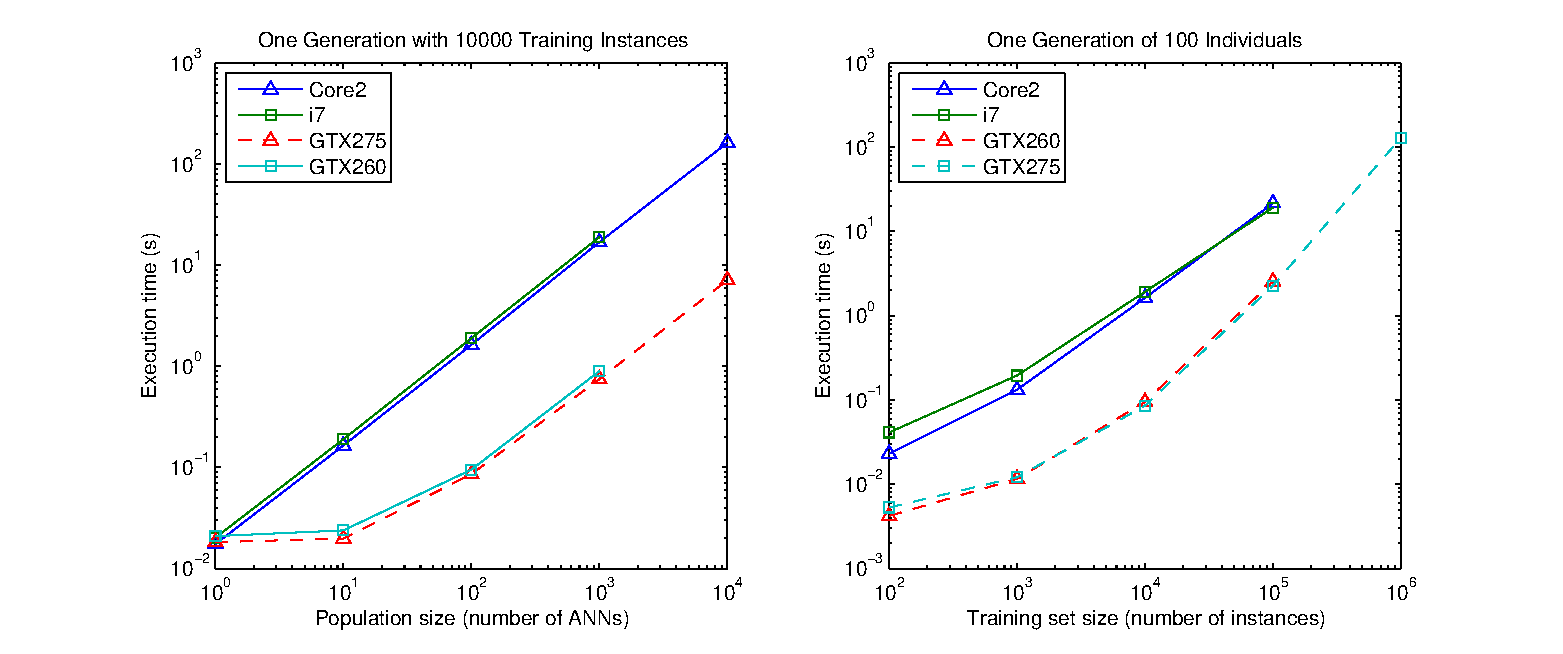
\includegraphics[width=\textwidth]{fig-performance}
	\caption{Training performance as a function of population size (left) and training set size (right). Note logarithmic axes.}
	\label{fig:training-performance}
\end{figure}

% ----------------------------------------------------------------------------
\subsection{Classification Performance} \label{results}
% ----------------------------------------------------------------------------
The classifier was trained over 12000 generations; the fitness metric during this training was lift at 20\% calculated on a training set which consisted of 70\% of the data set, chosen at random during initialization.  After each generation, the candidate ANN with the highest fitness value was used to classify 100 random subsets of the hold-out data set (each consisting of exactly one half of the hold-out data set), and the average of the lift at 20\% of these classifications was recorded.  Figure~\ref{fig:evolution-lift} demonstrates experimental results across 12,000 generations of population 50. The final estimated lift is 4.51 out of a maximum lift of 5.

\begin{figure}[h]
	\centering
	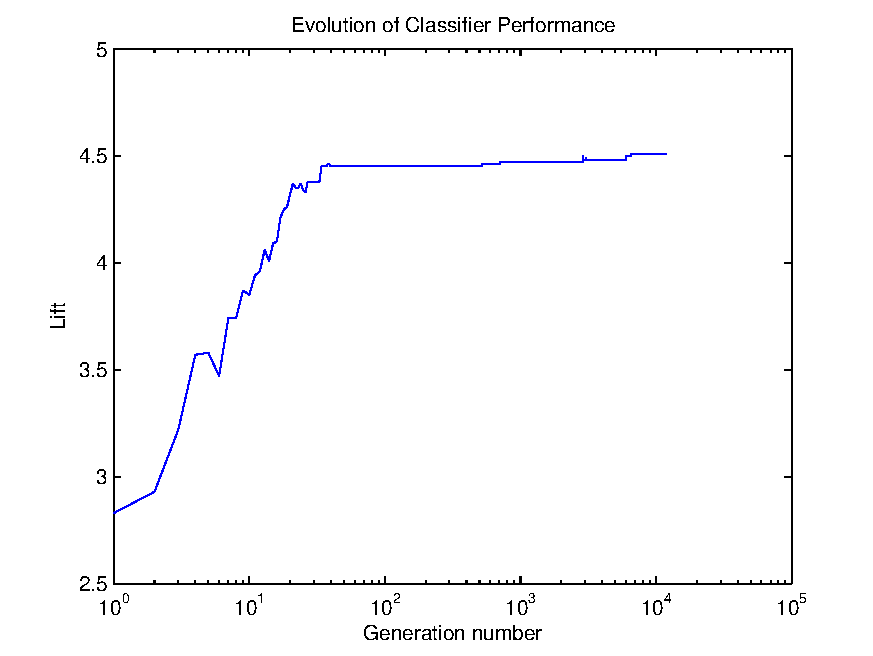
\includegraphics[width=0.5\textwidth]{fig-evolution-lift}
	\caption{Evolution of classifier lift. Note logarithmic generation number axis.}
	\label{fig:evolution-lift}
\end{figure}

When applied to the 2009 UC San Diego Data Mining Contest blind test data set, the resulting classifier produced a lift at 20\% value of 4.031, placing 35th in the world for classification of this data set. Due to the stochastic nature of genetic algorithms and the contest rules which state that contestants may test any number of candidate classifiers, it is likely that repeated entry into this contest would result in a higher ranking. The discrepency between the estimated performance and actual performance on the blind test data set can be attributed to the following:
\begin{itemize}
	\item Discrepency in test set size: the estimated performance measurements were done on sets of approximately 14000 patterns while the blind test data set has approximately 36000 patterns.
	\item Discrepency in class balance: when splitting the data set into training and hold-out data sets, class balance was not enforced for either of the sets. The blind test data set was known to have the same class balance as the given data set. Therefore, it is possible that the hold-out data set used to collect experimental results had a class balance which did not reflect the blind test data set.
	\item Nominal values unique to the blind test data set: It is possible that patterns with nominal values that do not appear in the training data set could cause misclassification, however, the pre-processing step which converts nominal values into numeric values accounts for values which have not been seen previously.
\end{itemize}

% ############################################################################
\section{Conclusion} \label{concl}
% ############################################################################
We have presented an implementation of GA training of feedforward ANN classifiers for the CUDA platform for GPU programming. By carefully designing memory organization, algorithm computational load and memory access patterns, we have obtained a 10-fold speedup compared to a conventional sequential CPU implementation. A multipass approach was required for part of our system to compensate for the limited amount of fast on-chip GPU memory. Our method scales across population and training set sizes and is expected to be useful in other data intensive machine learning and data mining tasks.

% ############################################################################
\section{Future Work} \label{future}
% ############################################################################
Montana and Lawrence \cite{GA-ANN} have demonstrated that a brief period of hill climbing after training with a genetic algorithm may increase the accuracy of classifier results. Thus, we could improve the accuracy of our methods by incorporating hill-climbing methods, such as the parallel backpropagation method described by Oei, Friedland and Janin \cite{backprop}.

In addition, parallelization methods of genetic algorithms involving multiple populations \cite{Alba1999} may interact favourably with data mining applications.  Seperate populations may be trained on different subsets of the training data, allowing for a more thorough search of the solution space which the training set presents.

% ############################################################################
% Bibliography
% ############################################################################
\bibliographystyle{unsrt}
\bibliography{bibliography}     %loads bibliography.bib

% ============================================================================
\end{document}
% ============================================================================
